% %%%%%%%%%%%%%%%%%%%%%%%%%%%%%%%%%%%%%%%%%%%%%%%%%%%%%%%%%%%%%%%%%%%%%%%%%%%%
\chapter{Dialogue modeling with less supervision}%
\label{chap:modeling}
% %%%%%%%%%%%%%%%%%%%%%%%%%%%%%%%%%%%%%%%%%%%%%%%%%%%%%%%%%%%%%%%%%%%%%%%%%%%%
Dialogue modeling is a complicated task requiring the ability to communicate in a natural language and handle discrete decision processes representing the conversation logic.
Various architectures have been proposed over the years (see Sections~\ref{02:ds-background},\ref{relwork:end-to-end}), mostly relying on explicit data annotation on multiple levels to guide the model training process.
One of the biggest challenges is to model task-oriented dialogue that requires interaction with external interfaces such as databases or API services.
This aspect puts a hard constraint on the dialogue system architecture -- it requires some explicit representation that allows one to communicate with external systems.
It's challenging to achieve this in a fully unsupervised setting due to the lack of model guidance in the form of structured labels.
However, we explore some of the approaches in this chapter.
First, we discuss the challenges of unsupervised task-oriented dialogue modeling in more detail in Section \ref{05:sec:to-unsup}.
Next, we propose our architecture that uses latent representations and explore its abilities and performance in Section \ref{05:sec:vrnn-model}.
Finally, we discuss the usage of pre-trained Language Models as dialogue models and try to answer whether these models can close the gap between unsupervised and supervised systems.
In this chapter, we present a modeling approach proposed by \citet{hudecek-dusek-2022-learning} and propose alternative extensions of another architecture using latent representations~\citep{lubis-etal-2022-dialogue}. 

\section{Challenges of TOD interaction with external interfaces under less supervision}
\label{05:sec:to-unsup}
There are multiple challenges to overcome when we try to model TOD without guidance in the form of labels (Section~\ref{02:no-super}).
This chapter addresses the challenges of action selection and interface interaction.
To enable the model to interact with external sources of information via API, we annotated points in the training dialogues where interaction with an external API is needed.
Therefore, the model can learn to construct the database queries ad-hoc using special outputs.
A turn-level annotation of database queries would represent a similar amount of annotation used in supervised training. It thus would not lead to our desired setting, where the model is trained without labeled data.
To support database access while avoiding costly turn-level annotation, we follow \citet{bordes2016learning} and 
insert sparse database queries and results into the training data, forming special dialogue turns.
Specifically, we identify turns that require database results, e.g.\ to inform about entity attributes or the count of matching entities, and insert a query-result pair in front of those turns (see Table~\ref{05:tab:example}). We argue that this is the minimal level of supervision required to operate a task-oriented system with database access successfully; it is significantly lower than the full dialogue-state supervision used by most systems.
Moreover, this kind of supervision is readily available in a realistic setting (such as using call center recordings and agent activity logs).
In practice, database queries are only inserted for 24\% turns on average.
Per-dataset query counts are 36\%, 23\%, and 11\% for CamRest676, MultiWOZ, and SMD, respectively.
Note that this approach still covers the task of an explicit state tracker since the necessary entity values are provided when needed.
Database query results can be stored and used in follow-up questions to maintain consistency.
.
\begin{table*}[tp]
    \centering\scriptsize
    \begin{tabular}{crp{0.6\linewidth}}
        \toprule
         \multirow{4}{*}{\bf Turn 1}&\bf user:& \texttt{Is there a \textbf{moderately priced} restaurant serving \textbf{italian} food anywhere in town?} \\
         &\bf system gold: & \texttt{query italian moderate} \\
         &\bf action: & \texttt{QUERY()} \\
         \midrule
        \multirow{4}{*}{\bf Turn 2}&\bf user/database:& \texttt{pizza express, Regent Street City Centre, 01223 324033, C.B 2, 1 D.B, centre}  \\
         &\bf system gold:& \texttt{Pizza express serves Italian food and is located in the town centre and is in the moderate price range .} \\        
        &\bf action: & \texttt{OFFER()} \\
         \midrule
        \multirow{4}{*}{\bf Turn 3}&\bf user:& \texttt{what is the \textbf{address} and \textbf{phone number} ?} \\
        &\bf system gold:& \texttt{their address is  Regent Street City Centre. Their phone number is 01223 324033. can I help with anything else ?} \\
         &\bf action: & \texttt{GIVE\_DETAILS()} \\
        \bottomrule
    \end{tabular}
    \vspace{-2mm}
    \caption{An example dialogue drawn from the CamRest676 validation set illustrates our injection of database interaction turns. We show the user input (or inserted database results), the gold-standard system response, and system action annotation based on manual rules. A database query is constructed in the first turn, and the second turn illustrates how the result is retrieved and fed as input. Values inferred correctly by our system are depicted in green.
    The wrong inference is in red.}
    \label{05:tab:example}
\end{table*}

\section{Task-Oriented dialogue with TO-VRNN}
The VRNN model architecture (see Section~\ref{02:sec:vrnn}) is designed to model sequences of observations coupled with latent states.
It's a generative model that can learn the conditional generative distribution of observations given the state.
Moreover, although VRNN does not require a fixed set of states, it can be adjusted to model discrete states.
The VRNN is great for modeling the discrete decision processes behind conversation exchanges, thanks to the above-mentioned properties.
However, we propose some extensions for task-oriented dialogue modeling to distinguish between the user and system roles and incorporate the possibility of handling interaction with external interfaces.
\begin{figure}[t]
    \centering
    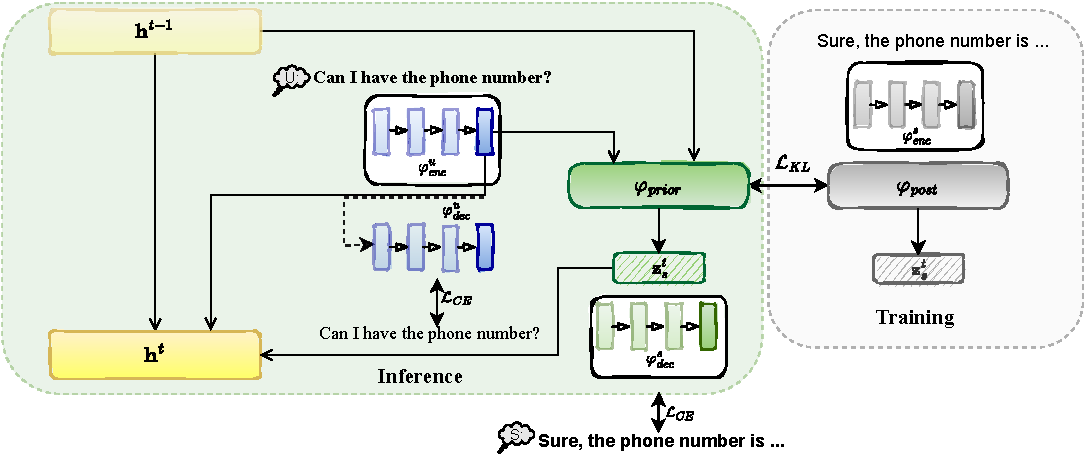
\includegraphics[width=0.9\textwidth]{images/vrnn-diagram.pdf}
    \caption{Visualization of our model architecture (one dialogue turn), described in Section~\ref{05:sec:vrnn-model}. Yellow boxes represent the turn-level VRNN's hidden state $h^t$. The user utterance is represented as the last hidden state of the encoder network $\varphi_{enc}^u$, which is trained as an autoencoder along with the decoder $\varphi_{dec}^u$. The system utterance, encoded by the network $\varphi_{enc}^s$, is an input to the posterior network $\varphi_{post}$ that helps to train the prior network $\varphi_{prior}$ to construct meaningful latent variables $\mathbf{z}_s$, which initialize the system utterance decoder $\varphi_{dec}^s$. The training uses the whole architecture, including the posterior network $\varphi_{post}$, while only the part shaded in green is used for inference. $\mathcal{L}_{CE}$ stands for cross-entropy loss, $\mathcal{L}_{KL}$ for KL-divergence loss.}
    \label{05:fig:vrnn_method}
\end{figure}

\subsection{TO-VRNN model description}
\label{05:sec:vrnn-model}
We extend the VRNN model introduced in Chapter \ref{02:sec:vrnn} to fit the task-oriented setup.
Figure \ref{05:fig:vrnn_method} depicts our model's architecture.
Following the original VRNN architectures (Section~\ref{02:sec:vrnn}), we employ a turn-level RNN that summarizes the context in its hidden state.
In each dialogue turn, we model user and system utterances with separate autoencoders to account for different user and system behaviors.
This contrasts with the original model described in~\ref{02:sec:vrnn}, which contains only one autoencoder in every time step.
We can divide the processing of one turn into two stages.
First, the user utterance, modeled with a standard vanilla autoencoder, is processed, and the last encoder hidden state $\varphi^u_{enc}(\mathbf{x}^t_u)$ provides the encoded representation used as an input for the next stage.

Next, the system part is used, which is realized by VAE with discrete latent variables $\textbf{z}_s$ conditioned on the context RNN's hidden state $\mathbf{h}^{t-1}$ and the user utterance encoding $\varphi^u_{enc}(\mathbf{x}^t_u)$.
The system module is trained as the VAE component in the VRNN model (\ref{02:sec:vrnn}) and creates latent representations interpreted as system actions.
This predicted latent variable is then used as an input to the system decoder that generates the realization of the latent action in the form of natural language.
Our model can thus be seen as a VRNN extended by an additional encoder-decoder module for input pre-processing.

To finalize the turn-processing step, we need to save the information into the turn-level network so it becomes part of the encoded context.
The turn-level network state update looks as follows:
\begin{equation}
    \begin{gathered}
        \mathbf{h}^{t+1} = \text{RNN}([\varphi^u_{enc}(\mathbf{x}_u^t),\varphi_{z}(\mathbf{z}^t_s)], \mathbf{h}^t)
    \end{gathered}
\end{equation}
In other words, we use representations from both user and system modules to pass the information necessary to update the overall state.

For word-level encoding and decoding modules ($\varphi_{enc}^u,\varphi_{enc}^s,\varphi_{dec}^u,\varphi_{dec}^s$), we use an RNN with LSTM cells.
We further experiment with attention \cite{bahdanau2014neural} over user encoder hidden states in the system decoder.
We train the model by minimizing a sum of the cross-entropy reconstruction loss on user utterances and the variational lower bound (Equation~\ref{eq:elbo}) on system responses.
\begin{equation}
\begin{split}
    \log~p(\mathbf{x}) \ge -\mathrm{KL}(q(\mathbf{z}|\mathbf{x})||p(\mathbf{z}))\\ + \mathbb{E}_{q(\mathbf{z}|\mathbf{x})}[\log~p(\mathbf{x}|\mathbf{z})]
    \label{eq:elbo}
\end{split}
\end{equation}
The final objective is presented in Equation~\ref{eq:loss-to-vrnn}.
There, $\phi$ and $\psi$ represent the parameters corresponding to system and user modules, respectively. $\mathbf{x}_s$ and $\mathbf{x}_u$ are system and user utterances and $\mathbf{u}$ is the encoded representation of the user utterance.
\begin{equation}
\begin{split}
    \mathbb{L}_{TO-VRNN}(\phi,\psi) = \mathbb{E}_{q_{\phi}(\mathbf{z}|\mathbf{x}_s)}[\log~p_{\phi}(\mathbf{x}_s|\mathbf{z})] \\
    -\mathrm{KL}(q_{\phi}(\mathbf{z}|\mathbf{x}_s)||p(\mathbf{z}))\\
    + log~p_{\psi}(\mathbf{x}_u|\mathbf{u})
\end{split}
    \label{eq:loss-to-vrnn}
\end{equation}
This objective directly extends the original training objective presented in \ref{02:sec:vrnn}.

When running in inference mode, only the prior distribution $p(\mathbf{z})$ is considered, which does not require the system utterance on the input.
Therefore, the model can generate the system response only with a user utterance on the input.

\paragraph{Latent Variables}
\label{05:sec:method_latent}
We use a set of $n$ \mbox{$K$-way} $(K=20;n=1,3,5)$ categorical variables to achieve good interpretability, following \citet{zhao2018unsupervised}.
This means that each variable is represented as a one-hot vector of length $K$, and we use $n$ such vectors.
Multiple ways exist to incorporate trainable discrete variables into a differentiable network (see Chapter~\ref{02:sec:vae_discrete}).
We use the Gumbel-Softmax distribution and the reparameterization trick \cite{jang2017categorical}.
We always take the item with the maximum probability concerning the predicted softmax distribution instead of sampling from it during inference.

\subsection{TO-VRNN Experiments}
In this section, we evaluate the quality of responses generated by our model.
We also inspect the model performance concerning dialogue success.
We focus on theoretical modeling and feasibility at this stage, which we believe is sufficiently demonstrated by corpus-based evaluation complemented by manual checks. Detailed interpretation of the learned representations follows in Section~\ref{05:sec:latents}.

\subsubsection{Data}
\label{05:sec:data}

We evaluate the model performance on three datasets: CamRest676 \cite{wen2016network}, MultiWOZ 2.1 (MW)\cite{budzianowski2018multiwoz,eric2019multiwoz} and Stanford Multidomain Dialogues (SMD) \cite{eric-etal-2017-key}
We use standard splits for MultiWOZ 2.1 and SMD.
We split CamRest676 in the 8:1:1 ratio, following previous work.
Detailed descriptions are given in Section \ref{02:sec:input-data-desc}.

\paragraph{Database queries} To include database information in the dialogues as described in Section~\ref{05:sec:to-unsup}, we first identify all turns in the original datasets where database information is required, using handcrafted rules.
These rules are very simple, and their creation requires minimal effort: whenever database results are provided in the data (based on simple pattern matches over system actions), we prepend a database query based on the ground truth state. The assumption is that these queries would naturally be available in a real-world scenario -- database queries induced by human operators can be logged along with client-operator conversations.
We then build database query turns based on the respective state annotation (see example in Table~\ref{05:tab:example}).
Note that database query parameters are the only annotation used to train our models apart from utterance texts; no other dialogue state annotation from the original datasets is used.

\subsubsection{Experimental Setup}
\label{05:sec:expe_setup}
We evaluate two versions of our model: one that uses the attention mechanism (\emph{attn}) and one without it (\emph{noattn}). The number and size of the variables are set based on a few cursory checks on the training data. Our models use ten latent variables by default; we discuss the influence of the number of latent variables in Table \ref{05:z_counts}.
Since our approach is the first to be evaluated in a task-oriented setting with minimal supervision, comparing it to prior works is difficult. Setups with full dialogue-state supervision are not comparable, and dialog-state metrics are not applicable without turn-level supervision. Therefore, we compare our models to standard architectures, such as vanilla LSTM or Transformer encoder-decoder, predicting sequentially using the same amount of supervision as our approach. We also compare to the HRED/VHRED models, perhaps the closest prior work to our approach. To put the results into perspective, we also include scores for fully supervised state of the art on our datasets.
However, note that these scores are not directly comparable.

\paragraph{Training details}
The model is trained with gradient descent using the ADAM optimizer.
We set the hyperparameters according to the BLEU and perplexity results of a grid search on the development set.
The utterance encoder and decoder hidden sizes are 250; the context-LSTM hidden size is 100.
The latent variables are 20-dimensional vectors; their number differs across experiments.
For the RNN components, we use a dropout probability of $0.3$.
The total model size is 7,047,529 parameters.
The training time is 3-8 hours using one GPU, depending on the dataset.
The training is sensitive to some parameters, such as the \nobreak{Gumbel-softmax} temperature, but otherwise, the model trains easily using conventional optimization methods.
To address the issue of posterior collapse (see Section~\ref{background:vae-problems}), we experiment with various approaches to KL annealing.
In our experiments, we use a liner annealing schedule, increasing the $\beta$ annealing coefficient from 0 $\rightarrow$ 1.
\paragraph{Metrics}
We use common metrics described in Table~\ref{05:automatic_metrics}).
To evaluate the quality of individual responses, we compute BLEU score and perplexity on the test set.
Without dialogue-state supervision, we cannot measure task-oriented metrics such \emph{joint goal accuracy}.
Therefore, we decided to measure dialogue success and entity match rate, which we adjusted to the minimally supervised case (details follow).
We also measure the database query accuracy.


\subsection{Results}
\subsubsection{Response quality}
Our architecture performs substantially better than (V)HRED, which commonly fails to acquire the necessary knowledge, especially on larger datasets.
The attention-based versions perform better on BLEU but lose slightly on perplexity.
Comparing HRED and VHRED shows that using the variational approach improves overall performance.
While the GPT-2 PLM outperforms our approach on perplexity, it is worse on BLEU score despite its huge capacity.

We compare to other relevant related works:
\begin{enumerate}
\item \citet{shi2019unsupervised} do not use their model for response generation, but they report a negative log-likelihood of approximately $5.5 \cdot 10^{4}$ when reconstructing the CamRest676 test set. Our \emph{TO-VRNN-noattn} model obtained $0.87 \cdot 10^{4}$, which suggests a better fit of the data.\footnote{This comparison is only approximate since the exact data split is not described by \citet{shi2019unsupervised} -- we can only use a test set of the same size, not the exact same instances.}
\item \citet{wen2017latent} measure response generation BLEU score on fully delexicalized CamRest676 data. Their best-reported result is 24.60, while our model gets 27.23 (30.10 with attention).
\end{enumerate}

Our models can generate relevant responses based on manual checks in most cases.
As expected, only the models, including database turns, can predict correct entities (cf.~Section~\ref{sec:emr}).
A relatively common error is informing about wrong slots, e.g., the model provides a phone number instead of an address or, even more frequently, provides wrong slot values (cf.~Table~\ref{05:tab:example-cont}).

\begin{table}[tp]
    \centering\footnotesize
    \begin{tabular}{l|c|rrrr|rrrr}
      \toprule
      model &  & \multicolumn{4}{c|}{\textbf{CamRest676}}  & \multicolumn{4}{c}{\textbf{MultiWOZ~2.1}} \\
      & db & BLEU & Ppl & MI & EMR &  BLEU & Ppl & MI & EMR \\
    LSTM & \textcolor{red}{\xmark} & 3.90 & 5.34 & -- & -- &  0.92 & 8.23 &
    -- & --\\
    Transformer & \textcolor{red}{\xmark} & 4.98 & 7.72 & -- & -- & 0.95 & 6.95 & -- & -- \\
    GPT-2 & \textcolor{red}{\xmark} & 15.40  & 1.18 & -- & -- & 9.40 & 2.77 & -- & -- \\
    GPT-2 & \textcolor{green}{\cmark} & 13.89 & 1.80 & -- & -- & 9.56 & 2.43 & -- & -- \\
    HRED & \textcolor{red}{\xmark} & \pz2.70 & 13.92 & -- & 0.02 & \pz2.98 & 29.61 &
    -- & 0.01\\
    VHRED & \textcolor{red}{\xmark} & \pz4.34 & 11.76 & 0.21 & 0.02 & \pz4.65 & 32.74 & 0.15 & 0.01 \\
    VHRED & \textcolor{green}{\cmark} & \pz8.50 & 10.23 & 0.17 & 0.36 & 3.82 & 16.61 & 0.07 & 0.04 \\
    \hdashline[0.5pt/2pt]
    TO-VRNN-noattn & \textcolor{red}{\xmark} & 12.98 & \pz4.64 & 0.29 & 0.01 & \pz7.18 & \pz9.16 & \bf0.42 & 0.02\\
    TO-VRNN-noattn & \textcolor{green}{\cmark} & 15.10 & \pz4.45 & \bf0.34 & 0.24 &  11.3 & \pz5.17 & 0.27 & 0.05\\
    TO-VRNN-attn & \textcolor{red}{\xmark} & \bf17.37 &\pz 5.07 & 0.16 &  0.09 & \bf12.28 & 10.19 & 0.06 & 0.04\\
    TO-VRNN-attn & \textcolor{green}{\cmark} & 17.10 & \pz\bf4.23 & 0.22 & \bf0.81 & 11.86 & \bf\pz6.03 & 0.05 & \bf0.08\\
    \hdashline[0.5pt/2pt]
    \emph{supervised $^{*}$} & \textcolor{green}{\cmark} & 25.50  & -- & -- & -- & 19.40 & 2.50 & -- & -- \\
    \bottomrule
  \end{tabular}
    \begin{tabular}{l|c|rrr}
      \toprule
      model &  & \multicolumn{3}{c}{SMD} \\
      & db & BLEU & Ppl & MI  \\
    LSTM & \textcolor{red}{\xmark} & 1.62 & 7.84 & -- \\
    Transformer & \textcolor{red}{\xmark}  & 1.53 & 6.33 & -- \\
    GPT-2 & \textcolor{red}{\xmark} & 9.26 & 2.46 & -- \\
    GPT-2 & \textcolor{green}{\cmark} & 4.54 & 2.02 & -- \\
    HRED & \textcolor{red}{\xmark} & \pz1.25 & 12.50 & -- \\
    VHRED & \textcolor{red}{\xmark} & \pz3.75 & 11.94 & 0.20 \\
    VHRED & \textcolor{green}{\cmark} & 3.94 & 11.86 & 0.19 \\
    \hdashline[0.5pt/2pt]
    TO-VRNN-noattn & \textcolor{red}{\xmark} & \pz7.35 & \pz6.18 & \bf0.53 \\
    TO-VRNN-noattn & \textcolor{green}{\cmark} & \pz9.24 & \pz\bf6.01 & 0.47 \\
    TO-VRNN-attn & \textcolor{red}{\xmark} & 12.30 & \pz6.36 & 0.04 \\
    TO-VRNN-attn & \textcolor{green}{\cmark} & \bf12.40 & 6.11 & 0.11 \\
    \hdashline[0.5pt/2pt]
    \emph{supervised$^{*}$} & \textcolor{green}{\cmark}& 14.40 & -- & --  \\
    \bottomrule
  \end{tabular}
  \caption{Model performance in terms of BLEU for generated responses, Perplexity (Ppl), and Mutual Information (MI) between the generated response and the latent variables $\mathbf{z}_s$. 
  We do not evaluate the database-enriched models on SMD as SMD's database structure does not map easily to our annotation style. 
  We measure MI only for the models that use latent variables explicitly. The \emph{db} column indicates systems that use database information. $^{*}$Note that the supervised state-of-the-art scores are not directly comparable, as the systems use full turn-level supervision.\cite{qin2020dynamic}; }
  \label{05:automatic_metrics}
\end{table}
\begin{table*}[tp]
    \centering\scriptsize
    \begin{tabular}{crp{0.6\linewidth}}
        \toprule
         \multirow{4}{*}{\bf Turn 1}&\bf user:& \texttt{Is there a \textbf{moderately priced} restaurant serving \textbf{italian} food anywhere in town?} \\
         &\bf system gold: & \texttt{query italian moderate} \\
         &\bf system hyp: & \texttt{query \textbf{\textcolor{darkgreen}{italian moderate}}}  \\
         \midrule
        \multirow{4}{*}{\bf Turn 2}&\bf user/database:& \texttt{pizza express, Regent Street City Centre, 01223 324033, C.B 2, 1 D.B, centre}  \\
         &\bf system gold:& \texttt{Pizza express serves Italian food and is located in the town centre and is in the moderate price range .} \\        
        &\bf system hyp:& \texttt{\textbf{\textcolor{red}{Pizza hut Cherry Hinton}} is a Italian restaurant in the \textbf{\textcolor{darkgreen}{centre}} part of town} \\
         \midrule
        \multirow{4}{*}{\bf Turn 3}&\bf user:& \texttt{what is the \textbf{address} and \textbf{phone number} ?} \\
        &\bf system gold:& \texttt{their address is  Regent Street City Centre. Their phone number is 01223 324033. can I help with anything else ?} \\
        & \bf system hyp:& \texttt{the phone number is \textbf{\textcolor{darkgreen}{01223 324033}}. Is there anything else I can help you with ?} \\
        \bottomrule
    \end{tabular}
    \vspace{-2mm}
    \caption{Predicted outputs or our VRNN model for a conversation snippet presented in~\ref{05:tab:example}}
    \label{05:tab:example-cont}
\end{table*}

\paragraph{Dialogue success}
The dialogue success or \emph{success rate} reflects the ratio of dialogues in which the system captures all the mentioned slots correctly and provides all the requested information.
We follow previous works \cite{nekvinda2021shades} and report corpus-based success scores instead of using a user simulator.
However, measuring success rate without turn-level labels is not straightforward.
We approximate tracking slot values turn-by-turn by checking for correct slot values upon database queries only, and we use this information to measure dialogue success.
Note that this is not equivalent to having state tracking labels available at all turns, but we consider it a reasonable approximation given our limited supervision -- database queries are crucial for presenting the correct entities to the user, which in turn decides the dialogue success.

The generated query attributes directly show the captured slots.


Success rate results are shown in Table~\ref{tab:success}.
Our system is not competitive with a fully supervised model but outperforms the baselines (VHRED, GPT).
Upon inspection,
we see that the system is often able to recognize correct slots.
However, it has difficulties capturing the correct values.
However, the scores are promising, considering the minimal supervision of our training.

\begin{table}[tp]
    \centering\small
    \begin{tabular}{lcc}
      \toprule
      model &  success & query acc.\hspace{-2mm} \\
      \midrule
      \multicolumn{3}{c}{\textbf{CamRest676}} \\
      \midrule
      VHRED & 0.21 & 0.91 \\
      TO-VRNN-noattn & 0.28 & 0.84 \\\hdashline[0.5pt/2pt]
      supervised SotA \cite{peng2021soloist}\hspace{-2mm} & 0.73 & N/A \\
      \midrule
      \multicolumn{3}{c}{\textbf{MultiWOZ}} \\
      \midrule
      TO-VRNN-noattn & 0.10 & 0.98 \\\hdashline[0.5pt/2pt]
      supervised SotA \cite{peng2021soloist}\hspace{-2mm} & 0.85 & N/A \\
      \bottomrule
  \end{tabular}
  \caption{Dialogue success and query accuracy comparison for VHRED, \emph{TO-VRNN-noattn} using the database and a state-of-the-art supervised system.}
  \label{tab:success}
\end{table}

\paragraph{Matching database entities}
\label{sec:emr}
Table~\ref{05:automatic_metrics} shows the performance of our models for entity matching.
We observe that the model performance without the database information is poor.
However, including the database information improves the performance substantially, especially in the case of CamRest676 data.
The MultiWOZ data is much more complex -- it contains more slots and multiple domains that can also be combined in an individual dialogue.
Nevertheless, we can still observe an improvement when we include the database queries.
We also note that using attention improves EMR substantially -- the latent variables alone cannot hold all information about particular values (cf.~Section~\ref{sec:pred_latents}).

\paragraph{Database query accuracy}
Further, we evaluate the accuracy of the database querying.
This metric measures if the system queries the database at appropriate turns.
The query's content is not considered in this case, as it is already considered in the success rate.
On MultiWOZ, we get a near-perfect accuracy, while our approach loses to VHRED on CamRest676 (see Table~\ref{tab:success}).
We hypothesize that different dialogue structures can cause such discrepancies among these two datasets.
The dialogues in CamRest676 usually contain just zero or one query during a dialogue, so our model might generate more queries than necessary.

\subsection{Latent Variable Interpretation}

\label{05:sec:latents}
\begin{table}[tp]
    \centering\small
    \begin{tabular}{l|ccc}
      \toprule
      & BLEU & Ppl & MI  \\
    \midrule
    TO-VRNN-noattn-1z  & 25.20 & 4.25 & 0.46  \\
    TO-VRNN-noattn-3z  & 26.80 & 4.24 & 0.26  \\
    TO-VRNN-noattn-5z  & 27.23 & 4.20 & 0.38  \\
    TO-VRNN-noattn-12z  & 29.83 & 4.12 & 0.35  \\    

    \bottomrule
  \end{tabular}
  %\vspace{-2mm}
  \caption{Evaluation of the model performance with different numbers of latent variables concerning automatic measures of BLEU, Perplexity (Ppl), and Mutual Information (MI) on the CamRest676 data.}
  \label{05:z_counts}
\end{table}
We believe that explaining and interpreting the model behavior is crucial, especially in a setting without full supervision.
Therefore, we design experiments to evaluate the model behavior and investigate whether the model captures salient dialogue features in the latent variables obtained during training on CamRest676 and MultiWOZ.
While the latent variables seem to be mainly useful for interpretability or structure induction, they are likely also contributing to the performance as smaller latent spaces yield lower performance, as shown in Table~\ref{05:z_counts}.

\subsubsection{Mutual Information}
Finally, we compute mutual information (MI) between the generated text and latent variables as well as among the latent variables themselves (see Table~\ref{05:automatic_metrics}).\footnote{
Since we measure MI between categorical variables, we quantize the continuous variables used in the VHRED model.}
We see that using attention dramatically affects the amount of MI between the latent variables and the generated text.
It appears that since attention bypasses the latent vectors, the decoder does not need to use them to store information.

\subsubsection{Clustering the actions}
\label{sec:clustering}
First, we want to assess whether similar variables represent similar actions.
We follow \citet{zhao2018unsupervised} and define utterance clusters according to the model's latent variables.
As a baseline, we consider random cluster assignment.
A stronger approach computes sentence representations using a BERT model tuned for sentence representations \cite{reimers-2019-sentence-bert} and then clusters the obtained sentence embeddings using K-means clustering.

We then use the homogeneity metric \cite{rosenberg-hirschberg-2007-v} to evaluate the clustering quality for the reference classes determined by manually annotated system actions (which are used for evaluation only).
Homogeneity reflects the information the clustering provides (and, by extension, the latent vectors used) and is normalized to the interval [0, 1].
The reason for choosing this metric is that it is independent of the number of labels and their permutations.
If all clusters only contain instances of a single class, we get the maximum homogeneity.

We provide the results in Table~\ref{tab:homo}.
The clusters formed on the CamRest676 data are more homogeneous than MultiWOZ, likely because of the greater dataset complexity in the latter case. 
In all cases, our clusters are much more homogeneous than clustering formed by random assignment.
We also compare favorably to a stronger baseline based on the clustering of the sentence representations.
These results suggest that the representations formed by our model correspond much better to the true actions seen in the data.

\begin{figure*}[t]
    \centering
    \includegraphics[width=0.70\textwidth]{images/dt2.pdf}
    \vspace{-5mm}
    \caption{A visualization of a decision tree trained on the CamRest676 data to predict a system action from the contents of the latent variables. Each node represents a decision based on one latent variable value, and the leaf node colors represent different system actions. When the condition in a given node is fulfilled, the algorithm proceeds into the right subtree, left otherwise. For clarity, we limit the maximum tree depth to 4. The limit slightly lowers the accuracy -- the pictured tree achieves an accuracy of 73\% on the CamRest676 data.}
    \label{fig:dt}
\end{figure*}

\subsubsection{Predictive power of the variables}
\label{sec:pred_latents}
\begin{table}[tp]
    \centering\small
    \begin{tabular}{l|c|cc}
      \toprule
      config & \textbf{CamRest676} & \multicolumn{2}{c}{\textbf{MultiWOZ 2.1.}} \\
       & gold & domain & action \\
      \midrule
      random  & 0.17 & 0.14 & 0.09 \\
      majority &  0.42 & 0.33 & 0.32 \\\hdashline[0.5pt/2pt]
      HRED & 0.65 & 0.45 & 0.44 \\
      VHRED & 0.52 & 0.36 & 0.32 \\
      GPT-2 & 0.65 & 0.60 & 0.55 \\
      %TO-VRNN-3z & 0.648 & 0.599 & 0.543 \\
      TO-VRNN-attn & 0.63 & 0.68 & 0.66 \\
%     TO-VRNN-5z (LR) & 0.721 &  & \\
      TO-VRNN-noattn & \textbf{0.75} &  \textbf{0.70} & \textbf{0.69} \\\hdashline[0.5pt/2pt]
      TO-VRNN-manual & 0.59 & -- & -- \\
      %10z (DT) & \textbf{0.759} & \textbf{0.641} & \textbf{0.404} \\
      %10z-attn (DT) & 0.597 & 0.460 & 0.296 \\

      \bottomrule
  \end{tabular}
  \caption{Accuracy of the domain and action decision-tree classifiers based on latent variables. 
  For details about the manual annotation process, see Section~\ref{sec:manual}.}
  \label{tab:latent_classification}
\end{table}
To evaluate the predictive power of the obtained latent representations, we train a simple classifier that predicts the system action and current domain, using solely the obtained latent representations as input features.
CamRest676 data does not include system action annotation.
Hence, we manually designed a set of rules to determine system actions.
An example of this rule-based action annotation is shown in Table~\ref{05:tab:example}.
For MultiWOZ, we predict both system action and the domain of the utterance.

To put our results into perspective, we include several baselines: trivial random and majority class baselines and classifiers using representations obtained with other methods (HRED, VHRED, GPT).
We use a decision tree (DT) classifier trained with the CART algorithm\footnote{\url{https://scikit-learn.org/stable/modules/tree.html}} and the \emph{gini} split criterion due to its good interpretability.
The results are shown in Table~\ref{tab:latent_classification}.
Our classifier beats the random and majority baselines in all cases.
It also outperforms classification based on (V)HRED and GPT representations.
This demonstrates that our approach produces high-quality interpretable representations.
We also observe that using attention harms the performance of the action classifier as it makes it possible for the models to bypass the latent variables.
On CamRest676, the latent variables explain most of the annotated actions.
Overall, we can observe that any hidden state taken from some trained model can explain some portion of the data.
However, using our approach seems to perform better in this aspect.
We also notice the influence of the number of latent variables on the performance.
In general, increasing the number of latent variables leads to a substantial performance improvement, which suggests that all the variables contribute with relevant information (see Table~\ref{tab:latent_classification}).

The information about domains and system actions is stored in categorical variables and can be extracted by a simple classification model such as the decision tree, which allows us to interpret and explain the behavior of our model.
For illustration, in Figure \ref{fig:dt}, we plot a DT with limited depth that achieves 73\% accuracy when predicting the system action on the CamRest676 data.
The aim is that latent variables hold high-level information, such as intents, actions, or domains. This helps interpretability but is insufficient for generating appropriate and factually correct responses -- here, we need to incorporate correct slot values.
This detailed information is captured and carried over via the attention mechanism in \emph{TO-VRNN-attn}.
Potential alternatives are copy mechanisms \cite{lei2018} or delexicalization on the generated outputs \cite{henderson_robust_2014,peng2021soloist}.

\subsubsection{Manual interpretation}
\label{sec:manual}
To explore the interpretability of our representations even further, we manually annotate the latent variables to obtain a simple handcrafted classifier.
Specifically, we draw a set of pairs of utterances and corresponding latent representations from the validation set.
We present the discrete representation vectors to an expert annotator to assign an action that each vector represents based on the sampled utterances.
This way, we obtain a mapping from the space of latent vectors to actions.
We then apply this mapping to predict actions on the test set (the \textit{TO-VRNN-manual} entry in Table \ref{tab:latent_classification}).
Note that in this approach, we only allow assigning an action to a whole vector, unlike in the case of a decision tree classifier which can take individual components into account.
As the results show, this approach works well despite the above limitation.

\begin{table}[tp]
    \centering\small
    
\begin{tabular}{l|c|c|c}
      \toprule
      \textbf{Source} &\textbf{ CamRest action} & \textbf{MW action} & \textbf{MW domain} \\
      \midrule
      TO-VRNN-noattn & 0.65 & 0.34 & 0.39 \\
      sent-repr & 0.45 & 0.33 & 0.30 \\
      random & 0.20 & 0.02 & 0.01 \\
      \bottomrule
  \end{tabular}
  \caption{Homogeneity for \emph{TO-VRNN-noattn} configuration using the database vs.~a clustering of sentence representations and random baseline.}
  \label{tab:homo}
\end{table}

\section{Hierarchical Variational Model for TOD (HVTOD)}
A structured representation of utterances in the dialogue with dialogue acts (Chapter~\ref{02:sec:basics}) is hierarchical because it is a composition of several concepts that can constrain each other.
Specifically, each utterance is characterized on the top level by its domain.
Each domain is connected with some intents and system actions, typically further connected with certain slots.
To reflect this hierarchical nature of the dialogue acts, we thus need some model that would structure its representations accordingly.
Since we are interested in latent representations, VAE architecture is a good option thanks to reasons discussed in \ref{05:fig:vrnn_method}.

VAEs for hierarchical architecture were successfully applied in the computer vision domain \cite{vahdat2020nvae,li2020progressive}.
We take inspiration from these works and apply the hierarchical variational autoencoder architecture to the dialogue domain.
We hypothesize that this structure will allow the model to work with different levels of abstraction and thus represent the decision process more accurately and with greater detail.
Note that there is no guarantee that the learned representations in different layers will also differ.
We want to explore this question to see if the model can learn to leverage this structure by itself. 

\subsection{HVTOD model architecture}
\begin{figure}[h]
    \centering
    \includegraphics[width=0.9\textwidth]{images/HVTOD-full-noN.pdf}
    \caption{The architecture of our HVTOD model. The dialogue context is first processed with a recurrent network encoder to obtain a hidden representation. This representation then serves as an input to the hierarchical system of variational encoders stacked on each other. The latent variables are merged to form the decoder's initial hidden state.}
    \label{05:fig:HVTOD-full}
\end{figure}
The proposed HVTOD architecture is based on the LAVA framework (\cite{lubis-etal-2022-dialogue}, see Section~\ref{02:sec:lava}).
In LAVA, the authors propose an architecture that uses latent representations of dialogue actions computed with VAE.
They use context encoded with an RNN encoder as an input into the VAE.
We extend the architecture so that instead of just one VAE.
We use a set of VAEs stacked on top of each other to model the latent variables.
The overall model architecture is depicted in Figure~\ref{05:fig:vrnn_method}.
In the input, we have a set of dialogues $\mathcal{D}$ where each dialogue $d$ with $n$ turns consists is represented as a sequence of altering system and user utterances $d = (s_1,u_1,...,s_n,u_n)$.
Similarly to LAVA, our model encodes the context $C^t = (s_1,u_1,...,s_t,u_t)$ with RNN-based utterance encoder to obtain a hidden representation of the context $h_0 = RNN_{\varphi_{enc}^u} (C^t)$.
The obtained representation $h_0$ is subsequently used as input to a hierarchical $L$ variational autoencoder system.
The autoencoders are stacked on each other.
Therefore, we refer to $l-th$ VAE as VAE on level $l$ or sometimes just \emph{layer l}.
Formally, each level $l$ computes parameters of posterior distribution $q(z_l|C^t)$ to sample the latent variable as follows:
\begin{equation}
\begin{split}    
    \mathbf{h}_l = e_l(\mathbf{h}_{l-1}) \\
    \mathbf{z}_l~\mathtt{\sim}~p(\mathbf{z}_l|C^t) = q_l(\mathbf{h}_l) \\
\end{split}
\end{equation}
where $e_l, A_l$ are trainable matrices.
In other words, each latent variable $z_l$ on level $l$ is sampled from a  distribution conditioned on context and preceding VAE layers $q(z_l|C^t,h_1,...,h_{l-1})$.
We use Gumbel-softmax distribution to obtain discrete vectors similar to the previous section.
To form the output, we aggregate the information on each layer in an output variable $g_l$ as follows:
\begin{equation}
\mathbf{g}_l = D_l(z_l) + \alpha \cdot \mathbf{g}_{l+1}, \alpha_l \in [0, 1]
\end{equation}
Where $\alpha_l$ is a scaling coefficient increased during training. All $\alpha_l$ are set to 1 in the trained network.
The output from the bottom hidden layer $g_1$ generates the response $s_{t+1}$  using an RNN decoder parametrized by $\varphi^s_{dec}$.

\subsection{HVTOD training}
In the LAVA framework, there are multiple stages of training.
Here, we want to focus on unsupervised pre-training with an auto-encoding objective.
However, we also evaluate the model performance in a supervised setting to understand the behavior better.
\begin{figure}[h]
    \centering
    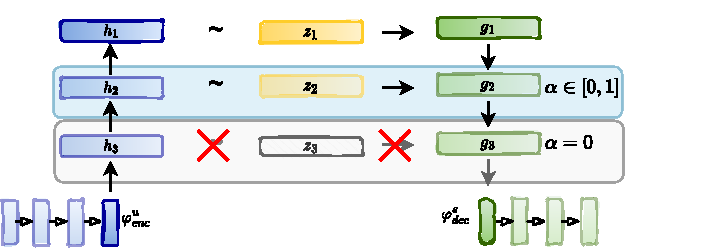
\includegraphics[width=0.9\textwidth]{images/HLAVA-fadein.pdf}
    \caption{Our hierarchical variational model during training. At this stage, the top layer is used completely; the second layer is faded-in with increasing coefficient $\alpha$ while the bottom layer is not used yet, so it is effectively disconnected from the computation graph.}
    \label{05:fig:HVTOD-fadein}
\end{figure}

\subsubsection{Training stages}
We start the training with autoencoding.
For the auto-encoding pre-training, we take an utterance $x$ as input and follow the traditional approach to VAE training.
We minimize the Evidence Lower Bound objective (ELBo), which we extend to reflect multiple levels of VAEs.
The full minimalization objective, therefore, is:
\begin{equation}
    \mathbb{L} = \mathbb{E}_{q(z_1|X^1),...,q(z_L|X^L)}[log~p(x|z_1,...z_L)] - \mathlarger{\mathlarger{\sum}}_{l=0}^L~D_{KL}[q(z_l|X^l)||p(z)]
\end{equation}
Where $X^L = x,z_1,...,z_{L-1}$.

The second stage is fine-tuning the pre-trained model.
We assume that the pre-training task helps to learn the network to create useful representations that can contribute to additional stages of training.
To confirm this, we employ the second stage of training in which we use supervision in the form of belief state labels, which we include in the input.
While in the autoencoding (AE) stage, the model learns to reconstruct the input utterance.
During fine-tuning (FT), the model takes dialogue context and predicts a system response.
FT stage utilizes the decoder pre-trained in the AE stage, and the encoder part is trained from scratch.

\subsubsection{Training specifics}
Training the network comprising multiple VAEs is challenging due to VAE training issues (Section~\ref{02:sec:vae}).
To simplify the training process, we incorporate the layers one by one.
Only the bottom layer is initially trained; more layers are added later.
To achieve this, we introduce a \emph{fade-in coefficient} $\alpha$~\citep{li2020progressive} that is being annealed from $0 \rightarrow 1$ over a predetermined number of steps and serves to incorporate a new layer during training smoothly.
This process is depicted in Figure~\ref{05:fig:HVTOD-fadein}.

Furthermore, we experiment with an additional training objective -- placeholder predictions.
Since we work with delexicalized data, we can train the network to predict which placeholders are present in the utterance.
We include this additional pseudo-supervision in the form of so-called \emph{placeholder loss} $\mathbb{L}_{pl}$, which is computed simply as binary cross-entropy for each placeholder prediction.

\subsection{Experiments}
We are interested in evaluating two aspects of the proposed model.
First, we explore how the multi-layer architecture contributes to the overall performance.
Next, we evaluate the properties of learned latent variables.
We use MultiWOZ 2.1 (See~\ref{02:sec:data-desc}) for training and evaluation.
We delexicalize (see Section~\ref{02:delex}) the utterances for training.

\subsubsection{Unsupervised HVTOD}
The second stage of HVTOD training, the fine-tuning, needs labels as supervision.
We are interested in the task of dialogue response generation when no labels are available.
Therefore, we also train an unsupervised variant of the model.
We base this stage on the auto-encoding objective and employ the same mechanism as auto-encoding but train the model to predict the next response instead of reconstructing it.

\subsubsection{Technical Details}
For training the model, we use a single GPU, NVIDIA A30.
We train the model for 100 epochs using the ADAM optimizer while we observe a decline in the validation loss.
The learning rate is set to $10^{-3}$.
We use discrete latent variables of dimension 20 to represent latent dialogue actions.
We determined the parameters by empirical experiments using grid search.
To get a fair comparison, we adjust the number of latent variables used according to the number of layers in the model hierarchy.
We adjust the number so that each configuration effectively has the same dimension of the latent space.
In the supervised training stage, we represent the belief state as a one-hot discrete vector corresponding to specific slots.

\subsubsection{HVTOD performance}
We evaluate the performance of HVTOD with a different number of layers and with or without the placeholder loss for dialogue response generation in unsupervised (Table~\ref{05:tab:hvtod-unsup}) and supervised (Table~\ref{05:tab:hvtod-ft}) setting.
All variants are first trained with an autoencoding objective.
We also evaluate the model quality after pre-training in Table~\ref{05:tab:hvtod-ae}.

Note that when we increase the number of layers, we decrease the dimension of the latent space accordingly.
Therefore, all the compared models have the same number of parameters.

\paragraph{Autoencoding}
We can see that in the autoencoding setting (Table~\ref{05:tab:hvtod-ae}), the increased number of layers helps to improve the performance concerning dialogue success and BLEU.
Moreover, the dialogue success is also improved by including our additional placeholder loss.

\paragraph{Supervised fine-tuning}
The results of supervised fine-tuning are given in Table~\ref{05:tab:hvtod-ft}.
This way, we achieve much higher scores, as expected.
Also, we can see that the placeholder loss contributes to the overall model performance as does the number of used layers.

\begin{table}[tp]
    \centering
    \begin{tabular}{c|c|c|c}
    \toprule
    \textbf{no layers}& \textbf{placeholder loss} & \textbf{Success-unsup} & \textbf{BLEU-unsup} \\
    \midrule
         1 & \textcolor{red}{\xmark} & 0.20 $\pm$ 0.06 & 15.36 $\pm$ 0.90 \\
         1 & \textcolor{green}{\cmark} & 0.34 $\pm$ 0.06 & 16.43 $\pm$ 0.62 \\
         2 & \textcolor{red}{\xmark} & 0.32 $\pm$ 0.07 & 16.39 $\pm$ 0.67  \\
         2 & \textcolor{green}{\cmark} & 0.33 $\pm$ 0.07 & 16.31 $\pm$ 0.45 \\
         3 & \textcolor{red}{\xmark} & 0.35 $\pm$ 0.03 &  16.67 $\pm$ 0.48 \\
         3 & \textcolor{green}{\cmark} & 0.35 $\pm$ 0.02 & 16.92 $\pm$ 0.84 \\
    \bottomrule
    \end{tabular}
    \caption{The results of HVTOD architecture after fine-tuning on dialogue response generation in an unsupervised setting, i.e. without belief state labels as inputs. We provide means and standard error intervals computed over five runs.}
    \label{05:tab:hvtod-unsup}
\end{table}

\paragraph{Unsupervised response generation}
For the unsupervised response generation (Table~\ref{05:tab:hvtod-unsup}), we observe the benefits of using the placeholder loss when only one-level hierarchy is used.
Surprisingly, we don't observe a similar effect when more layers are employed.
Nevertheless, there are performance gains when using placeholder loss in the supervised setting (Table~\ref{05:tab:hvtod-ft}).
This behavior shows that unsupervised dialogue response generation doesn't benefit from placeholder loss when more layers are employed.
This suggests that one of the layers in a multi-layer hierarchy can capture information that can be gained from placeholder loss.

\subsubsection{Latent space inspection}
We inspect the structure of the learned latent space by transforming the variables using the t-SNE algorithm~\cite{van2008visualizing} into 2-dimensional latent space and plotting them colored by their assignment to respective domains~\cite{lubis-etal-2022-dialogue}.
For autoencoding (Figure~\ref{05:fig:ae-layers}), the placeholder loss shapes the latent space to form more spread homogenous clusters, specifically on layer 1.
The same influence is even more visible when we visualize latent spaces after training the model for dialogue response generation (Figure~\ref{05:fig:ft-layers}).
Although the influence on latent space shape is clear, there is no significant difference in the final performance of the respective models.
We also observe that although each layer contains useful information, there is some overlap between the layers.
This suggests that it might be useful to enforce disentanglement of the latent variables somehow.

\begin{table}[tp]
    \centering
    \begin{tabular}{c|c|c|c}
    \toprule
    \textbf{no layers}& \textbf{placeholder loss} &  \textbf{Success-ft} & \textbf{BLEU-ft} \\
    \midrule
         1 & \textcolor{red}{\xmark} & 0.44 $\pm$ 0.08 & 17.37 $\pm$ 0.53 \\
         1 & \textcolor{green}{\cmark} & 0.52 $\pm$ 0.07 & 18.62 $\pm$ 0.52 \\
         2 & \textcolor{red}{\xmark} & 0.51 $\pm$ 0.03 & 19.17 $\pm$ 0.26 \\
         2 & \textcolor{green}{\cmark} & 0.55 $\pm$ 0.04 & 19.74 $\pm$ 0.36 \\
         3 & \textcolor{red}{\xmark} & 0.52 $\pm$ 0.04 & 19.36 $\pm$ 0.72 \\
         3 & \textcolor{green}{\cmark} & 0.55 $\pm$ 0.04 & 19.63 $\pm$ 0.41 \\
    \bottomrule
    \end{tabular}
    \caption{The results of HVTOD architecture after fine-tuning on dialogue response generation using belief state labels as inputs. We provide means and standard error intervals computed over five runs}
    \label{05:tab:hvtod-ft}
\end{table}

\begin{table}[tp]
    \centering
    \begin{tabular}{c|c|c|c}
    \toprule
    \textbf{No. of layers}& \textbf{placeholder loss}& \textbf{Success} & \textbf{BLEU} \\
    \midrule
         1 & \textcolor{red}{\xmark} & 0.46 $\pm$ 0.02 & 55.39 $\pm$ 1.43 \\
         1 & \textcolor{green}{\cmark} & 0.58 $\pm$ 0.03 & 55.86 $\pm$ 1.17 \\
         2 & \textcolor{red}{\xmark} & 0.50 $\pm$ 0.02 & 59.07 $\pm$ 1.31 \\
         2 & \textcolor{green}{\cmark} & 0.62 $\pm$ 0.01 & 62.42 $\pm$ 1.16 \\
         3 & \textcolor{red}{\xmark} & 0.53 $\pm$ 0.02 & 58.84 $\pm$ 1.46 \\
         3 & \textcolor{green}{\cmark} & \textbf{0.62} $\pm$ 0.01 & \textbf{64.50} $\pm$ 0.96 \\
    \bottomrule
    \end{tabular}
    \caption{The results of HVTOD architecture after pre-training with the unsupervised autoencoding objective. We provide means and standard error intervals computed over five runs. Note that dialogue success, in this case, indicates the reconstruction quality, but the model cannot be used for response dialogue generation since it's only trained on autoencoding.}
    \label{05:tab:hvtod-ae}
\end{table}


\begin{figure}[h]
\centering
\subfloat[level 1]{\label{sfig:a0}\includegraphics[width=.5\textwidth]{images/lava-tsne/ae-lvl-0-nll.png}}\hfill
\subfloat[level 1 + ph loss]{\label{sfig:b0}\includegraphics[width=.5\textwidth]{images/lava-tsne/ae-lvl-0-bce.png}}\\

\subfloat[level 2]{\label{sfig:a1}\includegraphics[width=.5\textwidth]{images/lava-tsne/ae-lvl-1-nll.png}}\hfill
\subfloat[level 2 + ph loss]{\label{sfig:b1}\includegraphics[width=.5\textwidth]{images/lava-tsne/ae-lvl-1-bce.png}}\\

\subfloat[level 3]{\label{sfig:a2}\includegraphics[width=.5\textwidth]{images/lava-tsne/ae-lvl-2-nll.png}}\hfill
\subfloat[level 3 + ph loss]{\label{sfig:b2}\includegraphics[width=.5\textwidth]{images/lava-tsne/ae-lvl-2-bce.png}}\\
\caption{Visualization of t-SNE projections of latent variables after the autoencoding stage, sorted left-to-right. In the bottom row, we have a version using the additional placeholder loss. The colors correspond to respective domains.}
\label{05:fig:ae-layers}
\end{figure}

\begin{figure}[h]
\centering
\subfloat[level 1]{\label{sfig:c0}\includegraphics[width=.5\textwidth]{images/lava-tsne/ft-lvl-0-nll.png}}\hfill
\subfloat[level 1 + ph loss]{\label{sfig:d0}\includegraphics[width=.5\textwidth]{images/lava-tsne/ft-lvl-0-bce.png}}\\

\subfloat[level 2]{\label{sfig:c1}\includegraphics[width=.5\textwidth]{images/lava-tsne/ft-lvl-1-nll.png}}\hfill
\subfloat[level 2 + ph loss]{\label{sfig:d1}\includegraphics[width=.5\textwidth]{images/lava-tsne/ft-lvl-1-bce.png}}\\

\subfloat[level 3]{\label{sfig:c2}\includegraphics[width=.5\textwidth]{images/lava-tsne/ft-lvl-2-nll.png}}\hfill
\subfloat[level 3 + ph loss]{\label{sfig:d2}\includegraphics[width=.5\textwidth]{images/lava-tsne/ft-lvl-2-bce.png}}\\
\caption{Visualization of t-SNE projections of latent variables after training for unsupervised dialogue response generation, sorted left-to-right. In the bottom row, we have a version using the additional placeholder loss. The colors correspond to respective domains.}
\label{05:fig:ft-layers}
\end{figure}

\subsection{Conclusion}
In this section, we introduced HVTOD, a hierarchical variational model for task-oriented dialogue.
We wanted to assess the contributions of hierarchical structure to the overall model performance.
Although the layer representations are not guaranteed to be distinct, we show that the model can leverage the benefits introduced by hierarchical structure since the variant with more layers outperforms the baseline (1-layer) variant with the same number of parameters.
The visualizations of latent spaces also uncover that the learned representations are structurally different.